\section{Data to the Cloud}
\label{sec:cloud}

There is a significant amount of data that is currently retained by
the controllers about water chemistry.  This includes historical
information on sensor readings (e.g., pH, oxidation-reduction potential (ORP),
free chlorine concentration, temperature, conductivity, turbidity,
alkalinity, etc.),
alarms (e.g., readings out of range, etc.), and user actions (e.g.,
set-point changes, etc.).
In addition, information on chemical stocks are frequently monitored
and logged as well.

It is currently possible to retrieve all of the above information from
a controller to a desktop application or mobile app by connecting to
the EZConnect server, providing appropriate authentication, and asking
the controller for its internal data logs.
The requests are made using a proprietary language that is
semantically limited (on purpose, for security
reasons~\cite{ezconnect,ccgss18}) to communicating the current
state as well as data logs for individual controllers.
This type of data request can result in both the console display of
Figure~\ref{console} as well as the plots of the data logs as shown
in Figure~\ref{graph}.

While these data can be quite useful, there are a pair of issues that
ultimately limit the impact that can be achieved.  First, the data
collection activity is triggered by the user.  While the controller
automatically maintains data logs, they are only delivered to a remote
location when a user makes a specific request to download the data.

Second, the data presentation is low-level.  By this we mean that
the data logs are presented in a reasonably viewable graphical presentation,
but there is little to no data analysis that is performed on the data.
It is up to the user to discern meaning from the data as presented.
Take, for example, the pH disturbance highlighted at noon over a 2~day
period (in Figure~\ref{graph}).  An immediate question that might come
to mind is, ``how general is this disturbance?'' It might be happening
at additional sites.  It might have happened only those two days, or it
might be part of a much longer trend.  Answering questions such as this require
the user to download data from other controllers, or other timeframes
on the same controller, all of which has historically been a manual,
user-initiated operation.

It is now possible to automatically
collect this information from a set of controllers (e.g., all
owned by an individual organization), retain the collected data in
the cloud, and realize benefit from the aggregation that is not realized
from each individual controller's data in isolation.

Owner/operators of this equipment are responsible for 
more than one controller, and they would benefit significantly from a relevant
summary view of the state of the water chemistry under their purview.
An example of a summary view (appropriate for each controlled body of water)
is illustrated in Figure~\ref{screenshot}.

\begin{figure}[htbp]
 \center
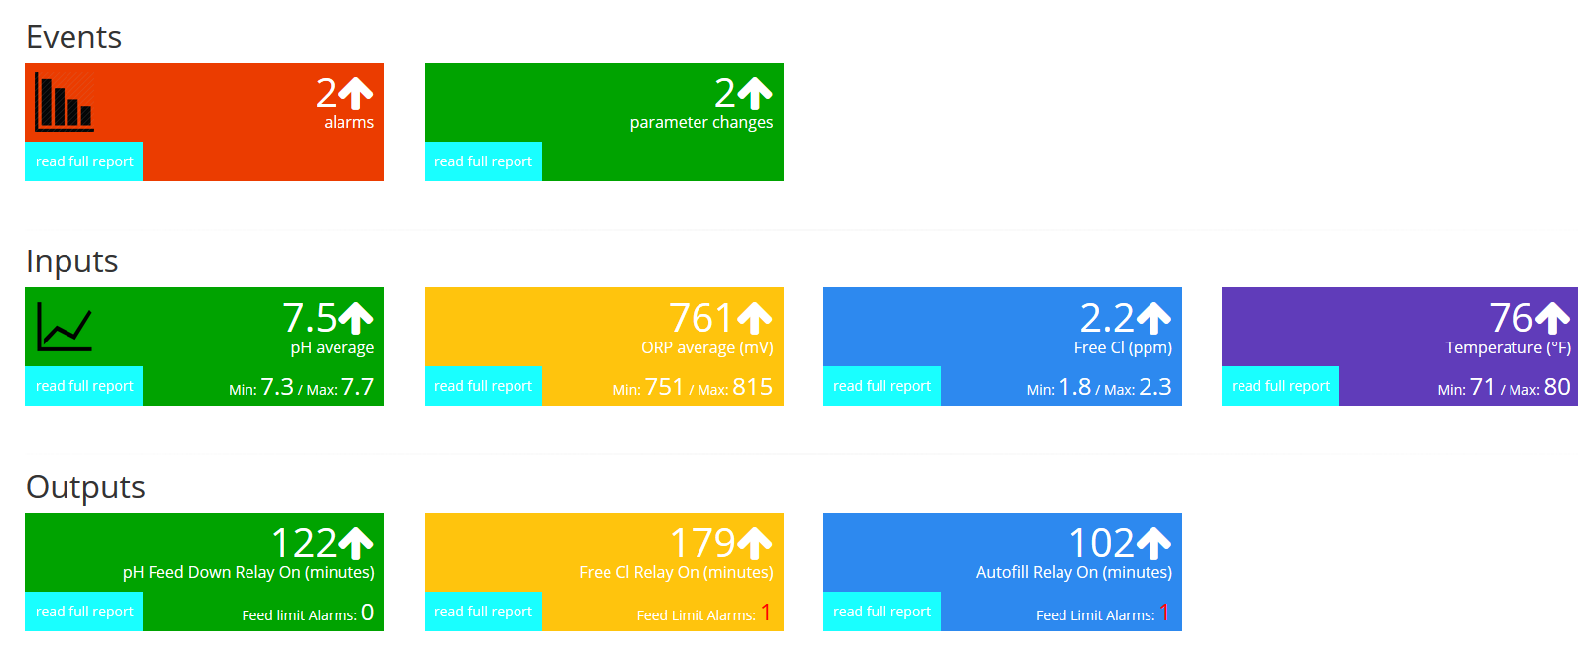
\includegraphics[width=\columnwidth]{screenshot}
    \caption{Screen capture of summary view data presentation. Additional
details are available via a link associated with each individual item.}
    \label{screenshot}
\end{figure}

In the figure, relevant information is organized for quick reference,
highlighting the ``big picture'' of the water chemistry, and allowing for
a more detailed drill down via a link associated with each item.
Groups of items are organized into categories (e.g., events, inputs,
outputs), and current values are supplemented with trends (indicated
by directional arrows) and ranges of values for the previous time period.

The above is facilitated by a number of concurrent processes running
on servers that are deployed in the cloud (see Figure~\ref{online}).
On the left, we see the elements from Figure~\ref{ezconnect}.
Applications can make a logical connection to individual controllers
via the EZConnect server.
In the center, the data server is executing a
data logging process that periodically communicates with each connected
controller (through the EZConnect server) and retrieves the data logs
for the immediate past period.
Those data are inserted into a persistent database, called the
controller database in the figure.
Finally,
a report generator mines the database to generate the information needed
for the summary views, and the summary view is served to the
user via a secure web server, called the BECSys Online server.
This latter server maintains the authorized users via an account
database.

\begin{figure}[htbp]
 \center
\includegraphics[width=\columnwidth]{EZAnalytics}
    \caption{EZAnalytics infrastructure. Each of the servers (and databases)
are deployed
in the cloud and can be replicated as needed to support increased capacity
and/or fail-over reliability.}
    \label{online}
\end{figure}

In the current instantiation, access to the EZAnalytics results (on the
right side of Figure~\ref{online}) are
made available to any device with a browser.  This is a distinction from
the access on the left side of the figure, which requires custom
software that understands the low-level specifics of each controller.
Removing the requirement for customized software is one of the ways
in which EZAnalytics is designed to be easier to learn and easier to use.
